\documentclass{amia_summit_2018}
\usepackage{graphicx}
\usepackage[labelfont=bf]{caption}
\usepackage[superscript,nomove]{cite}
\usepackage{color}
\usepackage{multirow}
\renewcommand*{\thefootnote}{\fnsymbol{footnote}}

\begin{document}

\title{Predicting the Outcome of Patient-Provider Communication Sequences using Recurrent Neural Networks and Probabilistic Models}

\author{Mehedi Hasan, BS$^{1}$\footnote[1]{Authors provided an equal contribution. \label{footnote1}}, Alexander Kotov, PhD$^{1}$\textsuperscript{\ref{footnote1}}, April Idalski Carcone, PhD$^{2}$, Ming Dong, PhD$^{1}$, Sylvie Naar, PhD$^{2}$}

\institutes{
$^1$Department of Computer Science, Wayne State University, Detroit, Michigan \\  
$^2$Department of Family Medicine and Public Health Sciences, School of Medicine, Wayne State University, Detroit, Michigan\\
}

\maketitle

\noindent{\bf Abstract}
\textit{The problem of analyzing temporally ordered sequences of observations generated by molecular, physiological or psychological processes to make predictions about the outcome of these processes arises in many domains of clinical informatics. In this paper, we focus on predicting the outcome of patient-provider communication sequences in the context of the clinical dialog. Specifically, we consider prediction of the motivational interview success (i.e. eliciting a particular type of patient behavioral response) based on an observed sequence of coded patient-provider communication exchanges as a sequence classification problem. We propose two solutions to this problem, one that is based on Recurrent Neural Networks (RNNs) and another that is based on Markov Chain (MC) and Hidden Markov Model (HMM), and compare the accuracy of these solutions using communication sequences annotated with behavior codes from the real-life motivational interviews. Our experiments indicate that the deep learning-based approach is significantly more accurate than the approach based on probabilistic models in predicting the success of motivational interviews (0.8677 versus 0.7038 and 0.6067 F1-score by RNN, MC and HMM, respectively, when using under-sampling to correct for class imbalance, and 0.8381 versus 0.7775 and 0.7520 F1-score by RNN, MC and HMM, respectively, when using over-sampling). These results indicate that the proposed method can be used for real-time monitoring of progression of clinical interviews and more efficient identification of effective provider communication strategies, which in turn can significantly decrease the effort required to develop behavioral interventions and increase their effectiveness.}

\section*{Introduction}
Temporally ordered sequences of discrete or continuous observations generated by molecular, psychological or psychological process(es) arise in many different areas of biology and medicine (e.g., DNA base-pairs, protein sequences, ECG measurements, laboratory results, diagnostic codes, utterances in the clinical dialog). Classification (or categorization) is a type of analysis of those sequences that has a broad range of important practical applications, from protein function \cite{yakhnenko2005discriminatively} or structure \cite{deshpande2002evaluation} prediction to detecting individuals with a heart disease \cite{wei2006semi}. Taking into account both the entire set of observations in a sequence, as well as the temporal order and potential dependencies between observations, makes sequence classification a more challenging task than a classification of independent observations. Predicting the outcome of those sequences (e.g. physiological or behavioral response) can also be viewed as a sequence classification problem.

In general, sequence classification methods fall into one of three major classes: feature-based, distance-based and model-based. Feature-based methods transform a sequence into a feature vector and apply a standard supervised machine learning method, such as Support Vector Machine \cite{leslie2004fast} or Decision Tree \cite{chuzhanova1998feature} to arrive at classification decision. The methods in this class have had limited success since traditional feature representation methods cannot easily account for the order of and dependencies between observations in a
sequence.

Distance-based methods classify a sequence by finding the most similar sequences with known classes based on a distance metric. The most commonly used distance metric is Euclidean distance with Dynamic Time Wrapping \cite{keogh2000scaling}. However, distance metrics are primarily designed for time series data, in which the observations are discretized by timestamps. The third type of sequence classification methods first creates a probabilistic model, such as the Markov Chain (MC) or Hidden Markov Model \cite{rabiner1989tutorial} (HMM), for sequences in each class based on the training data and then, classifies new sequences by applying the created models. While MCs and HMMs can capture first- and second-order dependencies between adjacent observations in a sequence, learning higher-order dependencies with these models requires prohibitively large amounts of data. By encoding sequences into low-dimensional representations, Recurrent Neural Networks (RNNs) are able to capture both short- and long-term dependencies and were shown to be effective at modeling different types of sequential data \cite{lipton2015critical}. Long Short-Term Memory (LSTM) \cite{hochreiter1997long} is a variant of RNNs, which successfully addressed the vanishing gradient problem \cite{bengio1993problem} of traditional RNN. LSTM demonstrated excellent performance in different domains, from speech \cite{graves2013speech} and handwriting recognition\cite{nion2013handwritten} to health informatics \cite{lipton2015learning, choi2016doctor}. Specifically, LSTM was used as part of a multi-label classification method to recognize patterns in multivariate time series of clinical measurements, such as body temperature, heart rate and blood pressure\cite{lipton2015learning}. LSTM was also effectively used for predicting the diagnosis and medication codes, given a sequence of codes from the previous patient visits \cite{choi2016doctor}. A further simplification and improvement of LSTM model, called the Gated Recurrent
Unit (GRU)\cite{chung2014empirical}, was later proposed. LSTM and GRU demonstrated markedly better performance among all other RNN variants for a variety of tasks in different domains.
  
In this paper, we address the problem of predicting the outcome of coded patient-provider communication (PPC) sequences in the context of the clinical dialog. Specifically, we focus on predicting the success (i.e. eliciting a particular type of patient behavioral response) of motivational interviews with obese adolescents and their caregivers based on an observed sequence of coded PPC exchanges during those interviews. Childhood obesity is a serious public health concern in the United States. Recent estimates indicate that approximately one-third (31.8\%) of U.S. children 2-19 years of age are overweight and 16.9\% are obese \cite{ogden2012prevalence}. Adolescents, who are obese, are likely to be obese in adulthood and have a greater risk of heart disease, type 2 diabetes, stroke, cancer, and osteoarthritis \cite{general2010surgeon}. One approach to effective obesity intervention is Motivational Interviewing (MI), an evidence-based counseling technique to increase intrinsic motivation and self-efficacy for health-related behavior change. The goal of MI is to encourage patients to explore their own desires, ability, reasons, need for and commitment to the targeted behavior change. These statements collectively referred to as ``change talk'' (CHT), consistently predict the actual behavior change\cite{apodaca2009mechanisms} that can be sustained for as long as 34 months\cite{walker2011influence} after an interview. However, the ability of providers to consistently elicit this type of patient communication requires knowledge of effective communication strategies for a variety of patients, which can only be obtained through analysis of a large number of annotated interviews. Since manual examination and analysis of MI interview transcripts is a very time-consuming process, designing effective MI interventions and tailoring them to particular populations can take years. Therefore, there is a need for informatics-based methods to facilitate the development of effective behavioral interventions, in general, and theoretically-grounded computational models to explore the mechanisms of MI's efficacy, in particular.

Our goal is to compare the accuracy of probabilistic models, such as MC and HMM, and deep learning methods, such as LSTM and GRU, for the task of predicting the success of clinical interviews (i.e. eliciting a particular type of patient behavioral response, such as CHT) at any point during a clinical interview based on a sequence of coded previous PPC exchanges in the same interview. This study is a continuation of our previous work \cite{kotov2015interpretable, hasan2016study}, in which we explored several machine learning methods for automatic annotation of clinical interview fragments with a large number of patient and provider behavior codes from a specialized codebook \cite{carcone2013provider}. While there have been some previous qualitative studies of patient-provider dialog in a clinical setting \cite{eide2004physician}, no previous work explored the applicability of state-of-the-art methods for sequence modeling to the analysis of PPC exchanges, in general, and predicting the desired patient behavioral response in the context of motivational interviews, in particular.

\section*{Methods}
\subsection*{\textit{Data collection}}

The experimental dataset for this work was constructed from the transcripts of 129 motivational interviews, which consist of a total of 50,239 segmented and annotated utterances. Each transcript corresponds to an MI interview session, which typically involves a counselor, an adolescent and a caregiver. The utterances were annotated based on the MYSCOPE codebook \cite{carcone2013provider}, in which the behavior codes are grouped into the patient (adolescent and caregiver) codes and the counselor codes. Annotated utterances were divided into successful and unsuccessful communication sequences. Successful communication sequences are the ones, which resulted in positive change talk (CHT+) or commitment language (CML+) statements by an adolescent or a caregiver, while unsuccessful sequences are the ones, which resulted in negative change talk (CHT-) or commitment language (CML-), or the ones, in which no change talk or commitment language statements were made. 

A fragment of an adolescent session transcript is presented in Table~\ref{tab:anno_examp}. In this example, $SS\rightarrow OQO\rightarrow HUPO\rightarrow OQTBN\rightarrow CHT+$ is a successful sequence, in which a counselor starts with an open-ended question and ultimately is able to elicit a positive change talk statement. As follows from this example, similar utterances, such as ``Yeah'' and ``Yes'', can be assigned different behavior codes (CHT+ and HUPW), depending on the context.\\

\begin{table}[h]
\caption{Fragment of the annotated transcript of a dialogue between a counselor and an adolescent. MYSCOPE codes assigned to the utterances and their meaning are shown in the first two columns.}    
\label{tab:anno_examp}
\centering
\begin{tabular}{|l|p{3.2cm}|l|p{8cm}|}
\hline
\bf{Code}  & \bf{Behavior} & \bf{Speaker} & \bf{Utterance} \\\hline
SS & Structure Session & Counselor & Okay. Can I meet with Xxxx alone for a few minutes? \\\hline
OQO & Open-ended question, other & Counselor & So, Xxxx, how you doing? \\\hline
HUPO &    High uptake, other    & Adolescent &    Fine \\\hline
OQTBN &    Open-ended question, target behavior neutral & Counselor &    That's good.  So, tell me  how do you feel about your weight? \\\hline
CHT+ &    Change talk positive    & Adolescent &    It's not the best. \\\hline
CQECHT+ & Closed question, elicit change talk positive & Counselor & It's not the best? \\\hline
CHT+ &    Change talk positive &    Adolescent & Yeah \\\hline
CQTBN &    Closed question, target behavior neutral  & Counselor &    Okay, so have you tried to lose weight before? \\\hline
HUPW &    High uptake, weight & Adolescent &    Yes \\\hline
\end{tabular}
\end{table}

The resulting experimental dataset was highly imbalanced. Out of 5143 observed sequences, 4225 or 82.15\% were positive and only 918 or 17.85\% were negative. No major differences were observed in the average length of successful (9.79 utterances) and unsuccessful (9.65 utterances) sequences.  

Since severely imbalanced datasets often distort the true performance of a classification method relative to a simple ``majority vote'' baseline (e.g. simply classifying every communication sequence as successful would result in 82.15\% accuracy on our dataset), it is important to properly address the class imbalance. We evaluated the performance of probabilistic and deep learning methods using both under-sampling and over-sampling for balancing the number of samples in different classes. Synthetic Minority Over Sampling Technique (SMOTE) \cite{chawla2002smote} is a widely used oversampling method for imbalanced datasets, in which new synthetic examples are generated for minority classes. Specifically, we generated synthetic examples at the borderline between the majority and minority classes \cite{nguyen2011borderline}. On the other hand, the under-sampling method reduces the number of samples in majority class by replacing the clusters of samples identified by the $k$-means clustering algorithm with the cluster centroids.

%Two MC and HMM models were trained, one model was trained on successful sequences, while another was trained on %unsuccessful sequences.  

\subsection*{\textit{Sequence classification methods}}
In general, a sequence can be viewed as a temporally ordered set of observations. In this study, an observation corresponds to a behavior code, which has a symbolic representation, such as $LUP+$ (low uptake, positive),
$OQECHT+$ (open-ended question, elicit change talk positive), etc.  Given a sequence of behavior codes $S_i = \{c_1, c_2,...,c_n\}$ representing PPC exchanges during some part of a motivational interview, the task of predicting interview success can be considered as sequence classification. Given a set of class labels $L = \{l_1, l_2,...,l_m\}$ (in our case, the labels are
``successful'' and ``unsuccessful'' motivational interview), a sequence classifier $C$ learns a function $S_i \to l_i, l_i \in L$ that maps a sequence $S_i$ into a class label $l_i \in L$.

Our proposed baseline prediction method consists of two steps. In the first step, we model successful and unsuccessful patient-provider interactions using first and second-order Markov Chain and
Hidden Markov Model, which are popular probabilistic models for discrete observation sequences with finite vocabulary. In the second step, we classify each test sequence based on the maximum
likelihood of generating that sequence from each model. Although HMM was originally developed for speech recognition \cite{rabiner1989tutorial}, it is one of the most widely used methods for sequence
modeling \cite{mutsam2016maximum, won2004training}. However, the latest advances in deep learning suggest that RNNs may provide better results than conventional machine learning methods for the task of
sequence classification. To verify this hypothesis, we employed two state-of-the-art variants of RNN in our experiments: Long Short-Term Memory (LSTM) \cite{hochreiter1997long} and Gated Recurrent Unit (GRU) \cite{chung2014empirical}.

\textbf {Markov Chain (MC)} is a probabilistic model that conditions each observation in a sequence only on preceding observation and not on any other past observation. First, we estimated two Markov models $M$ and $\overline{M}$, summarizing counselor strategies and patient responses, in the cases of successful ($M$) and unsuccessful ($\overline{M}$) motivational interviews. A
Markov model $M$ can be represented as a weighted directed graph $G = (V, E, p)$, in which:
\begin{itemize}
\item $V = \{CML+, CHT+, CHT-, AMB-, LUP+, LUP-, HUPW, OQO, CQTBN, CQECHT+,...\}$ is a set of vertices, consisting of adolescent, caregiver and counselor MI behavior codes;
\item $E \subseteq V \times V$ is a set of edges corresponding to possible transitions from one MI behavior code to the other in a sequence;
\item $p_M:E\rightarrow[0...1]$ is a function that assigns probability $p(c_i|c_j)$ to an edge between the MI behavior codes $c_i$ and $c_j$ based on the maximum likelihood estimation:
\begin{equation}
P_M(c_j|c_i) = \frac{n_{c_i,c_j}}{n_{c_i}}
\end{equation}
\end{itemize}
where $n_{c_i,c_j}$ and $n_{c_i}$ are the number of times a transition between the MI behavior codes $c_i$ and $c_j$ and the number of times the code $c_i$ have been observed in the training data, respectively. Given a Markov model $M$ (such that $S\subseteq V$), the probability that a sequence of MI behavior codes $S = \{C_1,...,C_N\}$ has been generated from a Markov model $M$ is:
\begin{equation}
P_M(S) = \prod_{i=2}^N p_M(c_i|c_1,\dots,c_{i-1})=\prod_{i=2}^N p_M(c_i|c_{i-1})
\end{equation}
In the second step, we quantify the likelihood of success of a given motivational interview at a certain time point given a sequence of MI behavior codes $S$ observed prior to that point as:
\begin{equation}
p(S\rightarrow successful) = \log\left(\frac{P_M(S)}{P_{\overline M}(S)}\right)= \sum_{i=2}^N \log p_M(c_i|c_{i-1})-\sum_{i=2}^N \log p_{\overline M}(c_i|c_{i-1})\label{eq:class}
\end{equation}
If $p(S\rightarrow successful) > 0 $, a communication sequence is predicted to be successful (i.e. result in positive change talk or commitment language). Otherwise, it is predicted to be unsuccessful.

The above model is also referred as first-order MC, since it only considers immediately preceding behavior code, when computing the state transition probabilities. In our experiment, we also considered second-order Markov model, which conditions each observation on the preceding two observations.  

\textbf {Hidden Markov Model (HMM)} is another probabilistic model used for modeling processes varying in time. HMMs are widely used for sequence analysis because of their ability to identify hidden states, corresponding to clusters of observations. Mathematically, HMM can be defined as $\lambda = (A, B, \pi)$, where:
\begin{itemize}
\item A is an $N\times N$ state transition probability distribution matrix $A = \{a_{ij}\}$
\item B is an $N\times M$ matrix $B = \{b_j(k)\}$ with observation symbol probability distribution for each state 
\item $\pi$ is the initial state distribution vector $\pi = \{\pi_i\}$
\end{itemize}
Hence, $N$ is a number of hidden states in the model and $M$ is a number of distinct observations per hidden state, i.e. the discrete vocabulary size. The key difference between HMM and MC is that HMM requires specifying the number of hidden states as a model parameter. HMM deduces a sequence of hidden states that best explains the observations along with the state transition probabilities and the distributions of observations (emission probabilities) per each hidden state. The Baum-Welch algorithm \cite{rabiner1989tutorial} is used to estimate the parameters of HMMs for successful and unsuccessful interviews using the corresponding training set, while the Viterbi algorithm \cite{rabiner1989tutorial} is used to determine the most likely sequence of hidden states for a given sequence of observations. After assignment of hidden states, the log-likelihood of success for an interview can be estimated using Eq.~\ref{eq:class} as well.

\textbf {Behavior code embeddings}. Representation of behavior codes was inspired by the recent success of word embeddings\cite{bengio2003neural}. Embedding is a representation of an object in low-dimensional space using a real-valued vector. In our study, embeddings of behavior codes were obtained as a by-product of training LSTM and GRU after feeding one-hot vectors as a representation of behavior codes as input to these RNNs. Behavior code embeddings have the property of representing similar codes with the vectors that are close to each other in low-dimensional space. Figure~\ref{fig:code_embedding} illustrates the MYSCOPE code embeddings visualized in 2-dimensional space by t-SNE \cite{maaten2008visualizing}. It can be seen that positive behavior codes such as OQECHT+, OQECML+, AF, AFL, SUP, RCML+S, CQECML+, etc. formed a cluster in the left part of Figure~\ref{fig:code_embedding}. The nearest neighbors of CQECML+ are highlighted by different color intensity (i.e. OQECML+ being more purple indicates that it is more similar to CQECML+). The right part of the figure demonstrates another cluster formed with negative behavior codes including CQECML-, AMB-, RCHT-C, OQECHT-, GINFO-, RBAC, LUP-, RCHT-S, RPTBC, RAMBC, AMB-, RCML-S, etc. It is interesting that the behaviors intended to elicit CHT+/CML+ group together, whereas the ones intended to elicit CHT-/CML- also group together and are located in the opposite regions of semantic space. 
    
\begin{figure}[!htb]
    \centering
    \includegraphics[width=0.50\textwidth]{figures/code_embed.eps}
    \caption{\textbf{2-D representation of behavior code embeddings}.}
    \label{fig:code_embedding}
\end{figure}

\textbf {Recurrent Neural Networks (RNN)} are a class of neural networks that have an internal memory, which makes them particularly suitable for processing sequences of observations. The ability of RNNs to capture long-term dependencies and remember past observations for predicting future observations is their main advantage over MCs and HMMs. These features are very useful in analysis of motivational interviews, in which any behavior observed at a particular point in the interview may be indicative of other behaviors that are observed later. In order to mitigate the vanishing gradient problem of earlier versions of RNN \cite{bengio1993problem}, Hochreiter et al.\cite{hochreiter1997long} proposed Long Short Term Memory networks (LSTM). There are several variants of LSTM model, among which the most notable one is the Gated Recurrent Unit\cite{cho2014properties} (GRU). GRUs are simpler than LSTMs and have been shown to be effective for a variety of Natural Language Processing tasks \cite{cho2014properties}. GRU is formally defined as follows:
\begin{equation}
z_t = \sigma(W_zx_t + U_zh_{t-1} + b_z)
\label{eq:firstgru}
\end{equation}
\begin{equation}
r_t = \sigma(W_rx_t + U_rh_{t-1} + b_r)
\label{eq:resetgru}
\end{equation}
\begin{equation}
\tilde h_t = tanh(W_hx_t + r_t \odot U_hh_{t-1} + b_h) 
\label{eq:candidategru}
\end{equation}
\begin{equation}
h_t = z_t \odot h_{t-1} + (1-z_t) \odot \tilde h_t
\label{eq:lastgru}
\end{equation}  
In Eq.~\ref{eq:firstgru}-\ref{eq:lastgru}, $\sigma$ corresponds to sigmoid function and $\odot$ designates an element-wise product. The update gate $z_t$ and reset gate $r_t$ at time step $t$ are computed by the Eq.~(\ref{eq:firstgru}) and~(\ref{eq:resetgru}), where $W_z$, $W_r$, $W_h$, $U_z$, $U_r$, $U_h$ are the weight matrices and $b_z$, $b_h$ and $b_r$ are bias vectors. The activation $h_t$ of the GRU at time $t$ is a linear combination of previous activation $h_{t-1}$ and the candidate activation $\tilde h_t$, which is represented by Eq.~(\ref{eq:lastgru}) and~(\ref{eq:candidategru}).
  
\begin{figure}[!htb]
    \centering
    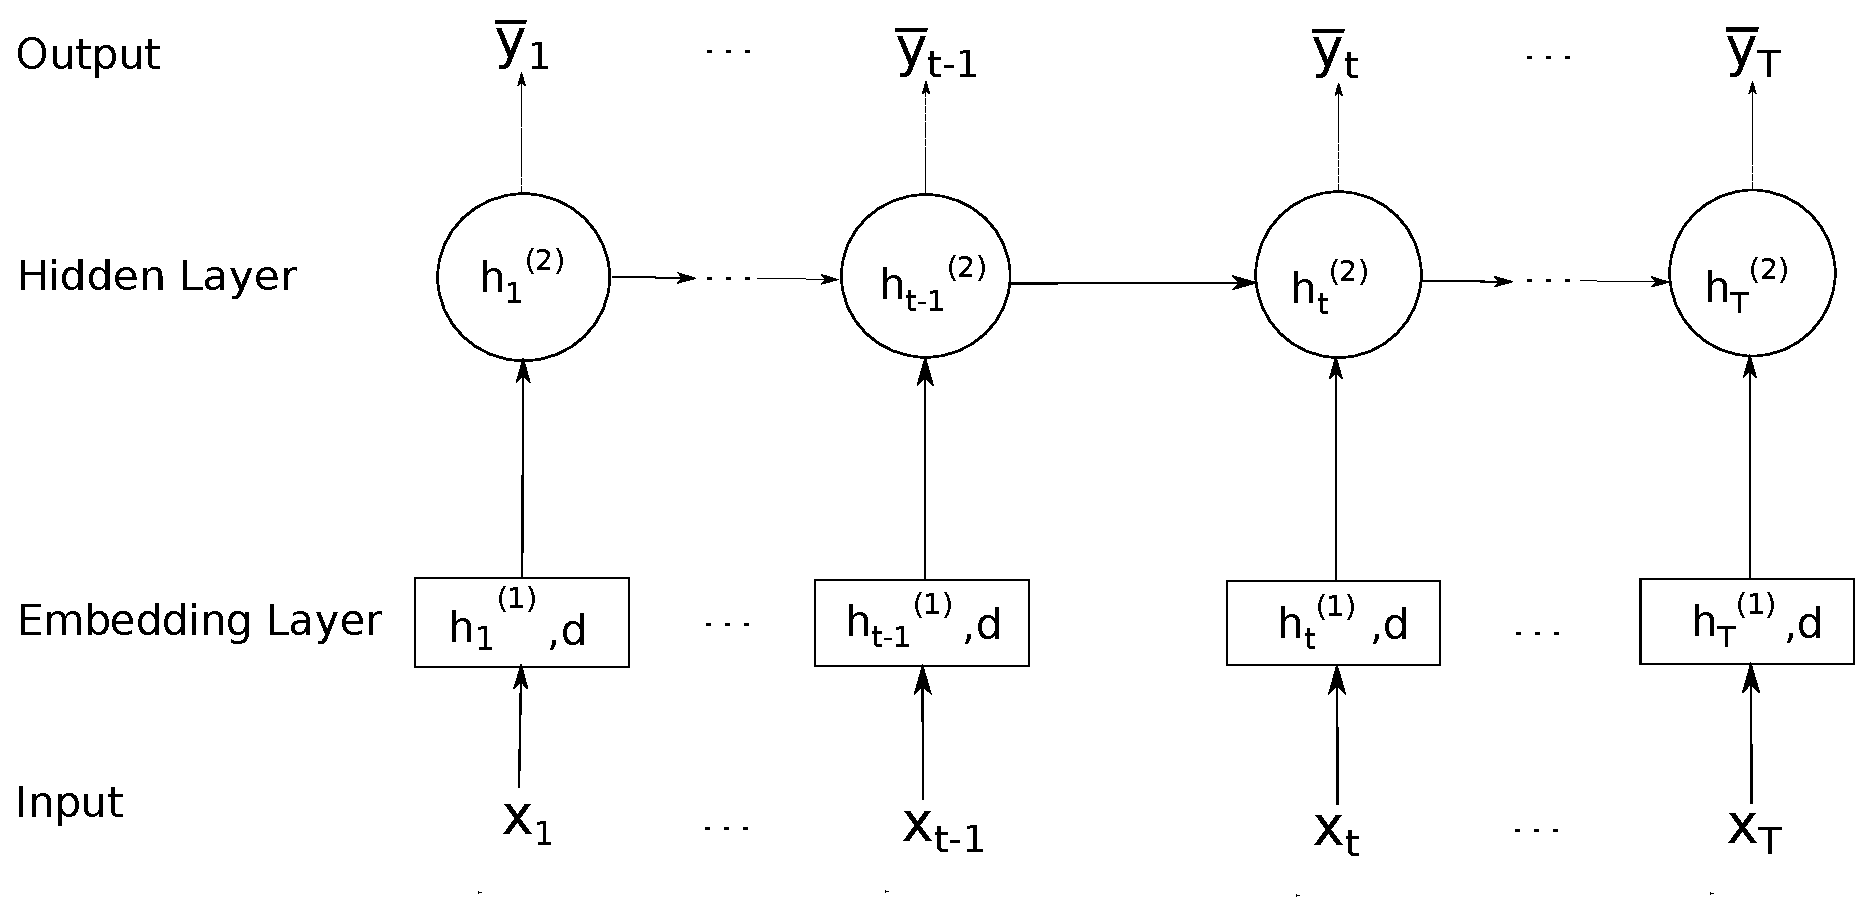
\includegraphics[width=0.70\textwidth]{figures/rnn_small.eps}
    \caption{\textbf{Proposed RNN model with target replication (TR)}.}
    \label{fig:rnn-model}
\end{figure}

The RNN architecture employed for sequence classification is shown in Figure~\ref{fig:rnn-model}. As can be seen from Figure~\ref{fig:rnn-model}, softmax is used at each time step to predict the class of a sequence observed so far. Since the sequence label is predicted at each observation, the proposed architecture is referred to as Recurrent Neural Network with Target Replication (TR). It is trained by minimizing the following hybrid loss function: 

\begin{equation}
\tilde{\mathcal{L}} = \alpha \cdot \frac{1}{T}\sum_{t=1}^T \mathcal{L}(\bar y^{(t)},y^{(t)}) + (1 - \alpha) \cdot \mathcal{L}(\bar y^{(T)},y^{(T)})
\label{eq:loss}
\end{equation}

As follows from Eq.~\ref{eq:loss}, the total loss $\tilde{\mathcal{L}}$ is a convex combination of the final loss $\mathcal{L}(\bar y^{(T)},y^{(T)})$ and the average loss over all observations in a sequence, where $T$ is the total number of observations, $\bar y^{(t)}$ is the output at step $t$, and $\alpha\ \epsilon\ [0, 1]$ is a hyperparameter controlling the relative importance of each loss type. We experimentally determined that the best performance is achieved when $\alpha=0.5$. Our model also contains several other hyperparameters, such as the number of embedding dimensions, the number of hidden units, learning rate, batch size, etc., which were optimized on the validation set. We implemented our models in Tensorflow with Adam optimizer as well as early stopping based on the validation loss and observed that our model converges after 100 epochs.    
  
\subsection*{\textit{Evaluation metrics}}
Performance of probabilistic and deep learning methods\footnote{the code for all models is publicly available at https://github.com/teanalab/myscope-sequential-analysis} was evaluated in terms of precision, recall, and F-measure using 10 folds cross-validation and weighted macro-averaging of these metrics over the folds. However, LSTM and GRU were trained on 80\% of the data and validated on 10\%, with the remaining 10\% of the data used for testing. 

%A true positive (TP) was counted when the method correctly classified a sequence into its actual class; a false positive (FP) was counted for a class when the method incorrectly classified a sequence into that class; a false negative (FN) for an actual class of sequence was counted when the method incorrectly classified the sequence into other class. The Precision of a class was defined as the ratio of the numbers of correctly classified sequences and all sequences identified as belonging to that particular class by the classifier (i.e Precision = TP / (TP + FP)). Recall of a class was defined as the ratio between the numbers of correctly classified sequences and all sequences of that particular class in the gold standard (i.e. Recall = TP / (TP + FN)). F-measure is computed as the harmonic mean of precision and recall (i.e. 2 x Precision x Recall / (Precision + Recall)). 

\section*{Results}
All sequence classification methods were evaluated in the case of both under and over-sampling. Predictive performance summary of all methods is summarized in Table~\ref{tab:result_under_over_sampled}.\\
 
\begin{table}[ht]
\centering
\caption{Performance of MC, HMM, LSTM and GRU with and without target replication (TR) for predicting the success of patient-provider communication sequences when under- and over-sampling were used to balance the dataset. The highest value for each performance metric is highlighted in bold.}
\label{tab:result_under_over_sampled}
  \begin{tabular}{|l|l|l|l|l|l|l|}
  \hline
   \multirow{2}{*}{\textbf{Method}} & \multicolumn{3}{|c|}{\textbf{Under-sampling}} & \multicolumn{3}{|c|}{\textbf{Over-sampling}} \\\cline{2-7}
   & \textbf{Precision}  & \textbf{Recall} & \textbf{F1-Score} & \textbf{Precision}  & \textbf{Recall} & \textbf{F1-Score}\\ \hline    
    
 Markov Chain $1^{st}$ Order & 0.7060 & 0.7044 & 0.7038 & 0.7932 & 0.7799 & 0.7775 \\ \hline
 Markov Chain $2^{nd}$ Order & 0.6395 & 0.6385 & 0.6379 & 0.7111 & 0.7029 & 0.7000\\ \hline
 Hidden Markov Model & 0.6244 & 0.6143 & 0.6067 & 0.7775 & 0.7567 & 0.7520\\ \hline
 LSTM & 0.8672 & 0.8626 & 0.8622 & 0.8411 & 0.8372 & 0.8368\\ \hline
 LSTM-TR & \textbf{0.8733} & \textbf{0.8681} & \textbf{0.8677} & \textbf{0.8424} & \textbf{0.8385} & \textbf{0.8381}\\ \hline
 GRU & 0.8674 & 0.8648 & 0.8646 & 0.8379 & 0.8342 & 0.8337\\ \hline
 GRU-TR & 0.8705 & 0.8676 & 0.8673 & 0.8412 & 0.8377 & 0.8373\\ \hline 
  \end{tabular}
\end{table}  

\subsection*{\textit{Predictive performance in the case of under-sampling}}
We used a small learning rate of 0.00005 and the batch size of 8 along with early stopping strategy for training deep learning models on the dataset balanced with under-sampling. Five major conclusions can be drawn from the results in Table~\ref{tab:result_under_over_sampled}. First, recurrent neural networks outperform probabilistic models and achieve 16.39\%-26.1\% higher F1-score. Second, LSTM with target replication has the best performance over all other RNN methods, and achieved F1-score 0.8677 with precision 0.8733 and recall 0.8681. Third, target replication strategy improves the performance of GRU and LSTM, with conventional GRU showing better performance than traditional LSTM. Fourth, among probabilistic models, the MC based method generally outperforms HMM across all metrics for under-sampled sequences. Fifth, second-order MC has lower precision, recall, and F-measure than first-order MC. In particular, precision, recall and F-measure decrease by 9.42\%, 9.36\% and 9.36\%, when going from first to second-order MC model.

\subsection*{\textit{Predictive performance in the case of over-sampling}}
Similar to the under-sampling scenario, early stopping strategy was also employed for training deep learning models on the dataset balanced with over-sampling. However, in this case, RNN models were trained with the learning rate of 0.00010 and the batch size of 55. Experimental results indicate that HMM had better performance than second-order MC, achieving 9.34\%, 7.65\%, and 7.43\% higher precision, recall, and F-measure, while HMM still had 1.98\%,
2.97\%, and 3.28\% lower precision, recall, and F-measure than first-order MC. Also similar to the under-sampling scenario, target replication improves the performance of RNN models and LSTM with target replication has the highest F1-score among all models. However, the predictive performance of LSTM and RNN decreases when over-sampling is used, while the performance of probabilistic models increases.

\begin{table}[ht]
\centering
\caption{Most likely communication sequences in successful and unsuccessful motivational interviews.}
\label{tab:common_patterns}
  \begin{tabular}{|l|l|}
  \hline
   \textbf{Type} & \textbf{Most likely communication sequences} \\ \hline      
successful & GINFO+: General information, positive $\rightarrow $ LUP+: Low uptake, positive $\rightarrow $ OQTBN: \\ 
& Open-ended question, target behavior neutral \\\hline
successful & SS: Structure session $\rightarrow $ GINFO+: General information, positive $\rightarrow $ CQECHT+: Closed-ended \\
& question, elicit change talk positive\\\hline
successful & SO: Statement, other $\rightarrow $ LUP+: Low uptake, positive $\rightarrow $ AF: Affirm $\rightarrow $ HUPW: High uptake, \\
& weight $\rightarrow $ OQECML+: Open-ended question, elicit commitment language positive. \\\hline
unsuccessful & ADV+: Advise, positive $\rightarrow $ AMB-: Ambivalence negative $\rightarrow $ OQECHT-: Open-ended \\
& question, elicit change talk negative\\\hline
unsuccessful & CQECHT+: Open-ended question, elicit change talk positive $\rightarrow $ RCHT-S: Reflect, change talk \\
& negative $\rightarrow $ OQECHT-: Open-ended question, elicit change talk negative \\\hline
unsuccessful & SUP: Support $\rightarrow $ AF: Affirm $\rightarrow $ CQTBN: Closed-ended question, target behavior neutral \\
& $\rightarrow $ OQECHT-: Open-ended question, elicit change talk negative $\rightarrow $ AMB-: Ambivalence negative\\\hline
  \end{tabular}
\end{table} 

\subsection*{\textit{Most likely communication sequences}}
Table~\ref{tab:common_patterns} provides examples of typical patient-provider communication sequences that frequently appear in successful and unsuccessful motivational interviews. We observed that in successful motivational interviews information is frequently provided using patient-centered communication (GINFO+) and structure session (SS) utterances, in which the counselor either explains the therapeutic agenda or attempts to transition to a new topic or session content. Sometimes, counselors also acknowledge the clients' communication or an off topic comment (SO). We also observed that affirmations (AF) and open-ended questions (OQECML+) have a strong effect on eliciting positive change talk or commitment language, which is consistent with MI theory. It can also be seen that providing advice using non-patient centered strategies (ADV-) leads to negative ambivalence (AMB-), which results in the interview heading in therapeutically wrong direction. Questions posed to elicit negative change talk or commitment language lead to CHT-, CML- or AMB-, which is  consistent with the manual analysis by clinicians.
%It can be seen that most successful sequence starts with a summary of the discussion or structured statement. After that, if adolescents express positive change talk, the counselor immediately reflects on that to reinforce adolescent's intrinsic motivation about behavior change. On the other hand, asking open- or closed-ended questions with eliciting negative change talk can lead to negative change talk, even in the cases when adolescents were showing a positive tendency in their previous communication. This observation can be explained by adolescents quickly confused when reiterating negative information that undermines their motivation. Analyzing such cases will allow the counselors to determine the negative information that can be discussed during the interviews.

\section*{Discussion}
By analyzing the experimental results of different communication sequence outcome prediction methods proposed in this paper, we arrived at the following conclusions. First, the overall predictive performance of RNN based methods is substantially higher than that of probabilistic models. In particular, the RNN-based methods achieve near-human accuracy for predicting the success of motivational interviews. This indicates that RNN is able to capture the structure of discourse in motivational interviews by preserving long-term dependencies among the behavior codes, which reflect the overall progression of the interviews. This provides evidence that RNNs are able to successfully replicate human cognitive processes to integrate previous information when making decisions. In addition to that, embeddings allow to reduce the dimensionality of codes in PPC sequences and consequently improve both precision and recall of  prediction.

Second, using target replication to compute the loss at each time step results in better performance for all configurations of the proposed RNN-based methods. This indicates that the average of the losses over all steps emphasizes the dependencies between the pairs of patient and provider codes, which results in more accurate estimates of the model parameters. Better estimates of parameters in RNN models of motivational interviews are propagated to the next step based on the relative importance of intermediate output, where they are aggregated into predictions for the entire sequence. This allows to achieve an improvement in prediction accuracy.

Third, using first-order Markov model results in better prediction accuracy compared to higher-order Markov models, which we attribute to the fact that the number of states in higher-order Markov models may grow exponentially with their order. As a result, accurate estimation of transition probabilities requires much larger training data. Using smaller datasets, which is the case when under-sampling is employed, will result in a sparsity problem, when many transitions are either not observed in the training set at all or observed only a few times, leading to missing or potentially inaccurate probability estimates. Obtaining large training sets cannot be easily accomplished in many domains, including motivational interviewing. In this study, we found out that using first-order Markov models is a reasonable trade-off between efficiency and accuracy.

Fourth, similar to traditional Markov model, HMM achieves a dramatic improvement in the prediction accuracy when larger training set is used. This indicates that sufficient training data is required to find the optimal settings of hyperparameters, such as the number of hidden states, initial state distribution, transition probabilities, and emission probabilities.   
 
Fifth, the proposed method can be used to identify the most effective communication strategies for eliciting a particular type of behavioral response. Awareness of these strategies by researchers can significantly decrease the time and effort required to develop effective interventions to address many public health conditions, such as childhood obesity, and tailor these interventions to particular patient cohorts. Awareness of these strategies by the counselors can lead to a greater success rate of motivational interviews.     
 
\section*{Conclusion}
In this paper, we compared the accuracy of Recurrent Neural Networks with Markov Chain and Hidden Markov Model for the task of predicting the success of motivational interviews. We found out that individual PPC exchanges are highly indicative of the overall progression and future trajectory of clinical interviews and can be used to predict their overall success. Our proposed methods can facilitate motivational interviewing researchers in establishing causal relationships between different communication strategies and the desired behavioral outcomes during the interviews without resource-intensive manual qualitative analysis of interview transcripts, which can significantly decrease the time and effort required to develop behavioral interventions. Our proposed methods can also help to identify the most likely sequences in successful and unsuccessful motivational interviews, which can directly inform clinical practice and increase the effectiveness of behavioral interventions. Our experimental results also indicate that the proposed methods can be used for real-time monitoring of the progression of clinical interviews. This work also has broad implications for public health research by providing a theoretically-grounded computational approach to qualitative data analysis.

\section*{Acknowledgments}
This study was supported by a grant from the National Institutes of Health, NIDDK R21DK108071, Carcone and Kotov, MPIs. We would like to thank the student assistants in the Department of Family Medicine and Public Health Sciences at Wayne State University School of Medicine for their manual annotation of experimental dataset with MYSCOPE codes. 

%\pagebreak

\bibliographystyle{vancouver}
\bibliography{references}

\end{document}